\section{Forwarder-Receiver}


Das Forwarder-Receiver design pattern stellt eine transparente Interprozess-Kommunikation für Softwaresysteme mit Peer-to-Peer Interaktionsmodell zur Verfügung. Es führt Forwarder und Receiver ein um die Peers von dem Kommunikationsmechanismus zu entkoppeln.

\subsection*{Example}


In einem Projekt hat ein Softwarenetwicklungsteam eine Infrastuktur für das Netzwerk-Management definiert. Das System besteht aus Agent-Prozessen welche auf jedem verfügbaren Netzwerk-Knoten (Node) laufen. Diese Agents sind verantwortlich für die Beobachtung und Überwachung von Ereignissen und Resourcen. Zudem erlauben sie Netzwerkadministratoren das Verhalten des Netzwerks zu verändern, zum Beispiel durch das Modifizieren der Routing-Tabellen. Um den Informationsaustauch und eine schnelle Propagation von Netzwerkbefehlen sicherzustellen ist jeder Agent mit Peer-to-Peer an andere Agents verbunden und handelt als Client oder Server - je nachdem was geforderet ist. Die Infrastruktur muss eine breite Palette von Hardware und Software unterstützen, wobei die Kommunikation nicht von der verwendeten Interprozess-Kommunikation abhängig sein darf.

\subsection*{Context}


Peer-to-Peer Kommunikation

\subsection*{Problem}


Ein verbreiter Weg um Verteilte Anwendungen zu erstellen ist es, low-level Interprozess-Kommunikation zu nutzen, wie TCP/IP, sockets oder Message Queues. Diese werden von fast allen Betriebssystemen zur Verfügung gestellt und sind sehr effizient im Vergleich zu high-level Mechanismen, wie Remote Procedure Calls.

Diese low-level Machanismen führen jedoch oft Abhängigkeiten zum darunterliegenden Betriebssystem oder verwendeten Netzwerkprotokollen ein.

\subsubsection*{Forces}


\begin{itemize}
	\item Das System soll die Austauschbarkeit des Kommunikations-Mechanismus erlauben.
	\item Die Kooperation von Komponenten entspricht dem Peer-to-Peer Model, bei dem der Sender nur den Namen des Empfängers kennen muss.
	\item Die Kommunikation zwischen Peers sollte keinen grossen Einfluss auf die Performance haben.
\end{itemize}

\subsection*{Solution}


Verteilte Peers arbeiten zusammen an einem bestimmten Problem. Ein Peer kann als Client, durch aufrufen von Services, oder als Server, durch zur Verfügungstellen von Services, oder als beides handeln. Die Details des verwendeten IPC-Mechanismus sind vor den Peers versteckt durch das Kapsseln der Funktionalität in eigene Komponenten.

\subsection*{Structure}

\begin{figure}[H]
	\centering
	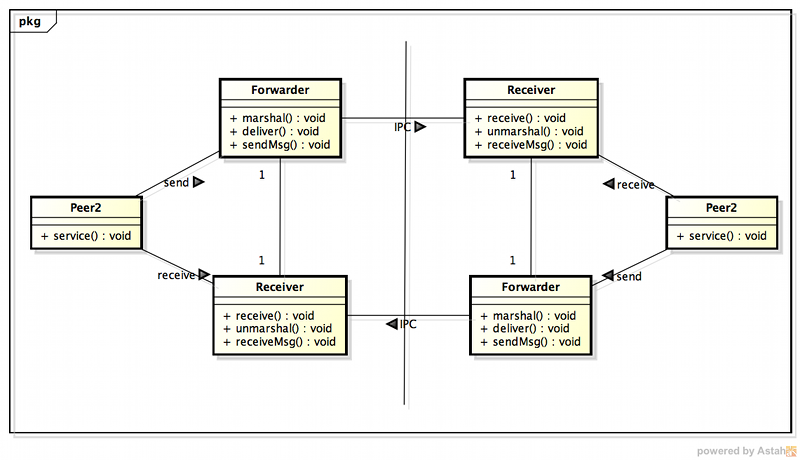
\includegraphics[width=0.7\textwidth]{content/posa1/images/forwarder-receiver-classes.png}
	\caption{Forwarder Receiver Klassendiagramm}
\end{figure}


Forwarder Kompontenen sendne Nachrichten über Prozessgrenzen. Ein Forwarder stellt eine Schnittstelle zur Verfügung welches eine Abstraktion eines bestimmten IPC-Mechanismus zur Verfügung stellt. Er enthält auch Funktionalität für das Marshalling. Zudem kann er Adressen von Namen physikalischen Adressen zuordnen.

Receiver Komponenten sind Verantwortlich für das Empfangen von Nachrichten. Ein Receiver stellt ebenfalls eine Schnittstelle zur Verfügung welches eine Abstratktion eines bestimmten IPC-Mechanismus zur Verfügung stellt. Wie der Receiver kümmert sich die Receiver Komponente auch entsprechend um das Unmarshalling.

\subsection*{Dynamics}

\begin{figure}[H]
	\centering
	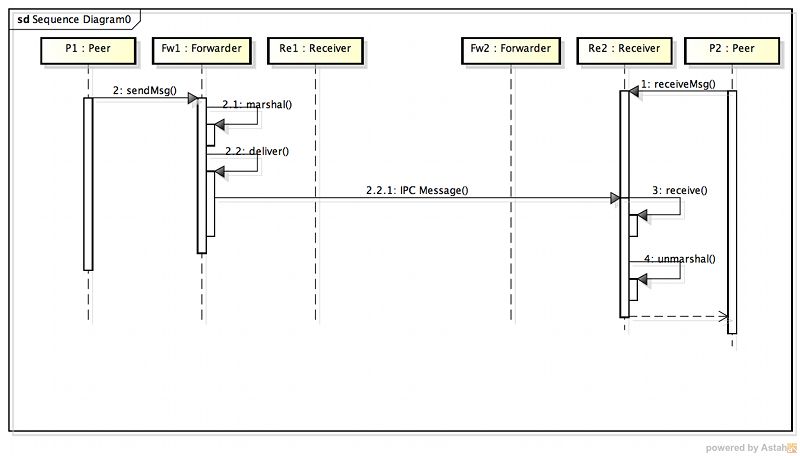
\includegraphics[width=0.7\textwidth]{content/posa1/images/forwarder-receiver-sequence.png}
	\caption{Forwarder Receiver Sequenzdiagramm}
\end{figure}


\begin{enumerate}
	\item P1 benögigt einen Serivce von P2. Dazu sendet er einen Request an seinen Forwarder Forw1 und gibt den Namen des Empfängers an.
	\item Forw1 bestimmt die physikalische Adresse des Remote-Peers und marshallt die Nachricht.
	\item Forw1 liefert die Nachricht an den Recv2 aus.
	\item Zu einem späteren Zeitpunkt bittet P2 seinen Receiver Recv2 auf einkommende Requests zu warten. Nun empfängt Recv2 die Nachricht von Forw1.
	\item Recv2 unmarshallt die Nachricht und gibt sie seinem Peer P2 weiter.
\end{enumerate}


\begin{enumerate}
	\item Spezifiziere ein Namen-zu-Adress-Mapping
	\item Spezifiziere ein Nachrichtenprotokoll
	\item Wähle einen Kommunikationsmechanismus.
	\item Implementiere die Forwarder. Forwarder müssen zudem über ein Repository verfügen um Adressen auflösen zu können. Dies kann statisch im Code implementiert sein oder dynamisch zur Laufzeit änderbar.
	\item Implementiere den Reiceiver. Receiver können blockierend oder nicht blockierend implementiert werden. Zudem muss entschieden werden, ob auf mehreren Kanälen kommuniziert werden kann oder nicht. Falls ja wird ein Demultiplexing benötigt.
	\item Implementiere die Peers. Es kann sowohl One-Way wie auch Two-Way Kommunikation umgesetzt werden.
	\item Implementiere eine Startup-Konfiguration. Insbesondere müssen Forwarder mit einem gültigen Name-to-Address mapping initialisiert werden.
\end{enumerate}


\begin{itemize}
	\item Forwarder-Receiver without name-to-adress mapping. Kann aus Performancegründen Sinn machen. Dabei muss der Peer am Forwarder die physikalische Zieladresse übergeben.
\end{itemize}

\subsection*{Known Uses}


\begin{itemize}
	\item TASC - Software Development Toolkit
	\item Reboot - Material Flow Control Software
	\item ATM-P
	\item BrouHaHa - Distributed Smalltalk Environment
\end{itemize}

\subsection*{Consequences}


\subsubsection*{Benefits}


\begin{itemize}
	\item Effiziente Interprozess-Kommunikation
	\item Kappselung von IPC
\end{itemize}

\subsubsection*{Liablities}


\begin{itemize}
	\item Keine Unterstützung für flexibles Re-Konfigurieren von Komponenten. Es besteht keine einfache Möglichkeit um die Verteilung von Peers zur Laufzeit anzupassen. Kann durch Dispatcher Kompontente gelöst werden, siehe Client-Dispatcher-Server Design Pattern.
\end{itemize}

\subsection*{See also}


\begin{itemize}
	\item Client-Disptacher Design Pattern
\end{itemize}


